\begin{figure}[t]
\centering\small
\begin{subfigure}[t]{0.32\linewidth}
  \centering
  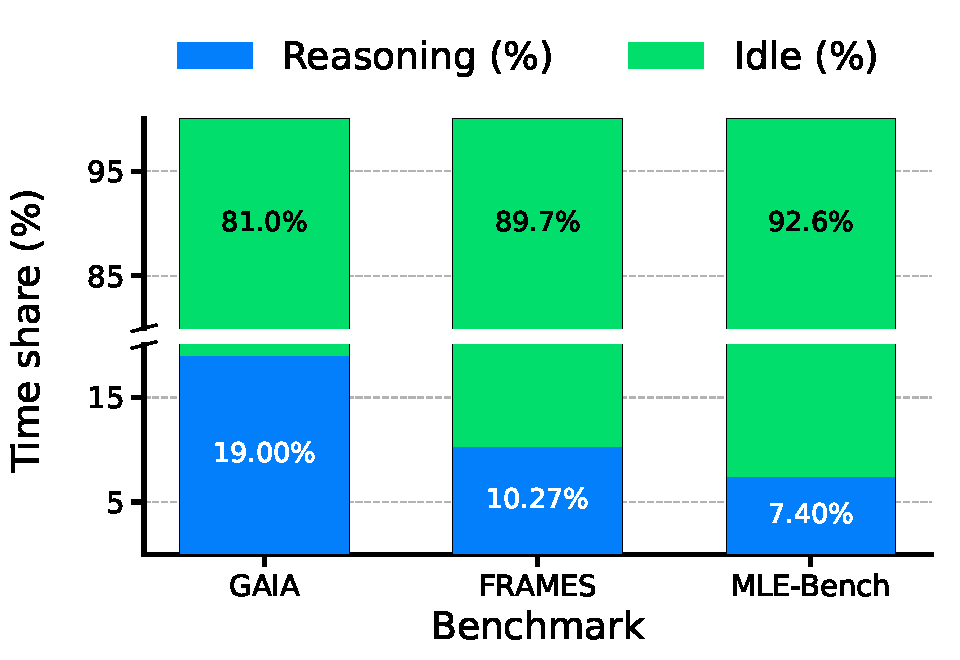
\includegraphics[width=\linewidth]{figures/observation_source_new.pdf}
  \caption{Idle vs.\ Reasoning Share}
  \label{fig:observation-source}
\end{subfigure}\hfill
\begin{subfigure}[t]{0.32\linewidth}
  \centering
  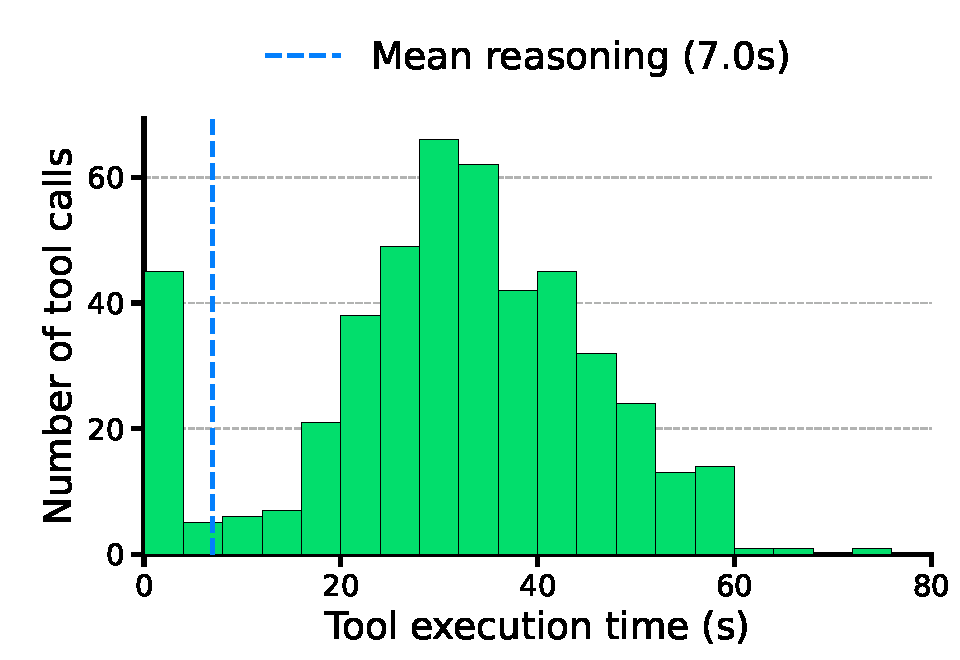
\includegraphics[width=\linewidth]{figures/observation_tool_execution_time_new.pdf}
  \caption{Tool Execution Time}
  \label{fig:observation-tool-execution-time}
\end{subfigure}\hfill
\begin{subfigure}[t]{0.32\linewidth}
  \centering
  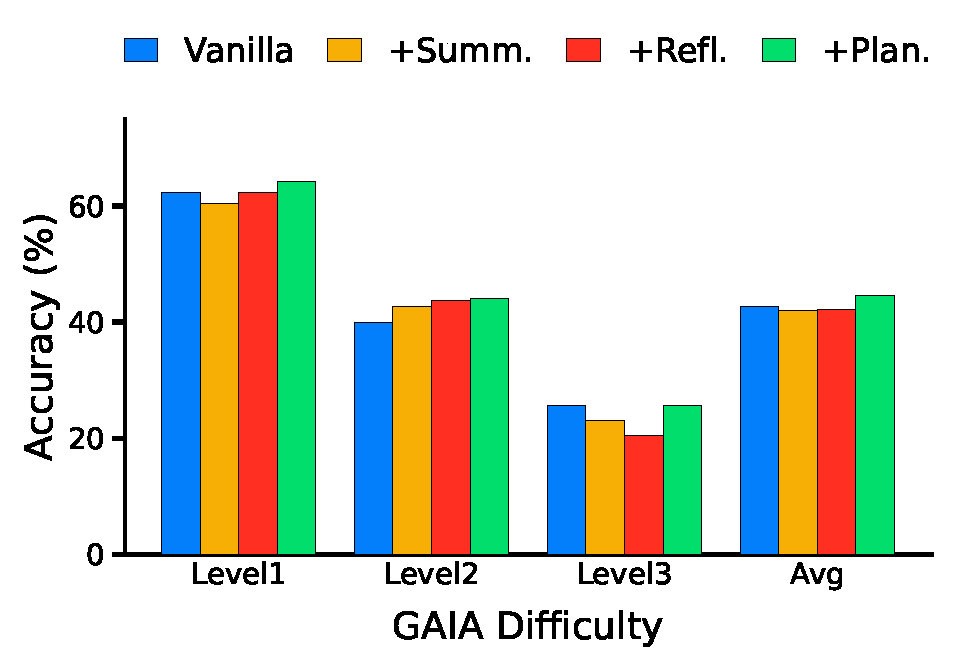
\includegraphics[width=\linewidth]{figures/observation_methods.pdf}
  \caption{Idle-Time Strategies}
  \label{fig:observation-methods}
\end{subfigure}
\caption{\textbf{How Can We Leverage Idle Time in LLM Agents?}
(a) Reasoning time vs.\ tool execution time (\ie idle time) across benchmarks.
(b) Histogram of per-call tool execution times. 
(c) Accuracy of three idle-time strategies (Summarization, Reflection, Planning) vs.\ vanilla.}
\label{fig:observation-idle}
\end{figure}
